%!TEX root = bachelor.tex
\chapter{Theoretische Grundlagen}
\label{ch:theory}

Rechtshändiges Koordinatensystem...

\section{Kegel}
\label{s:cone}

\begin{definition}[Kegel]
	kegel
\end{definition}

In der weiteren Arbeit betrachten wir nur gerade Kreiskegel

\begin{figure}[!htb]
	\centering
	\includegraphics[scale=.5]{images/fullCone.eps}
	\caption{Gerader Kreiskegel}
	\label{fig:cone}
\end{figure}

\begin{figure}[!htb]
	\centering
	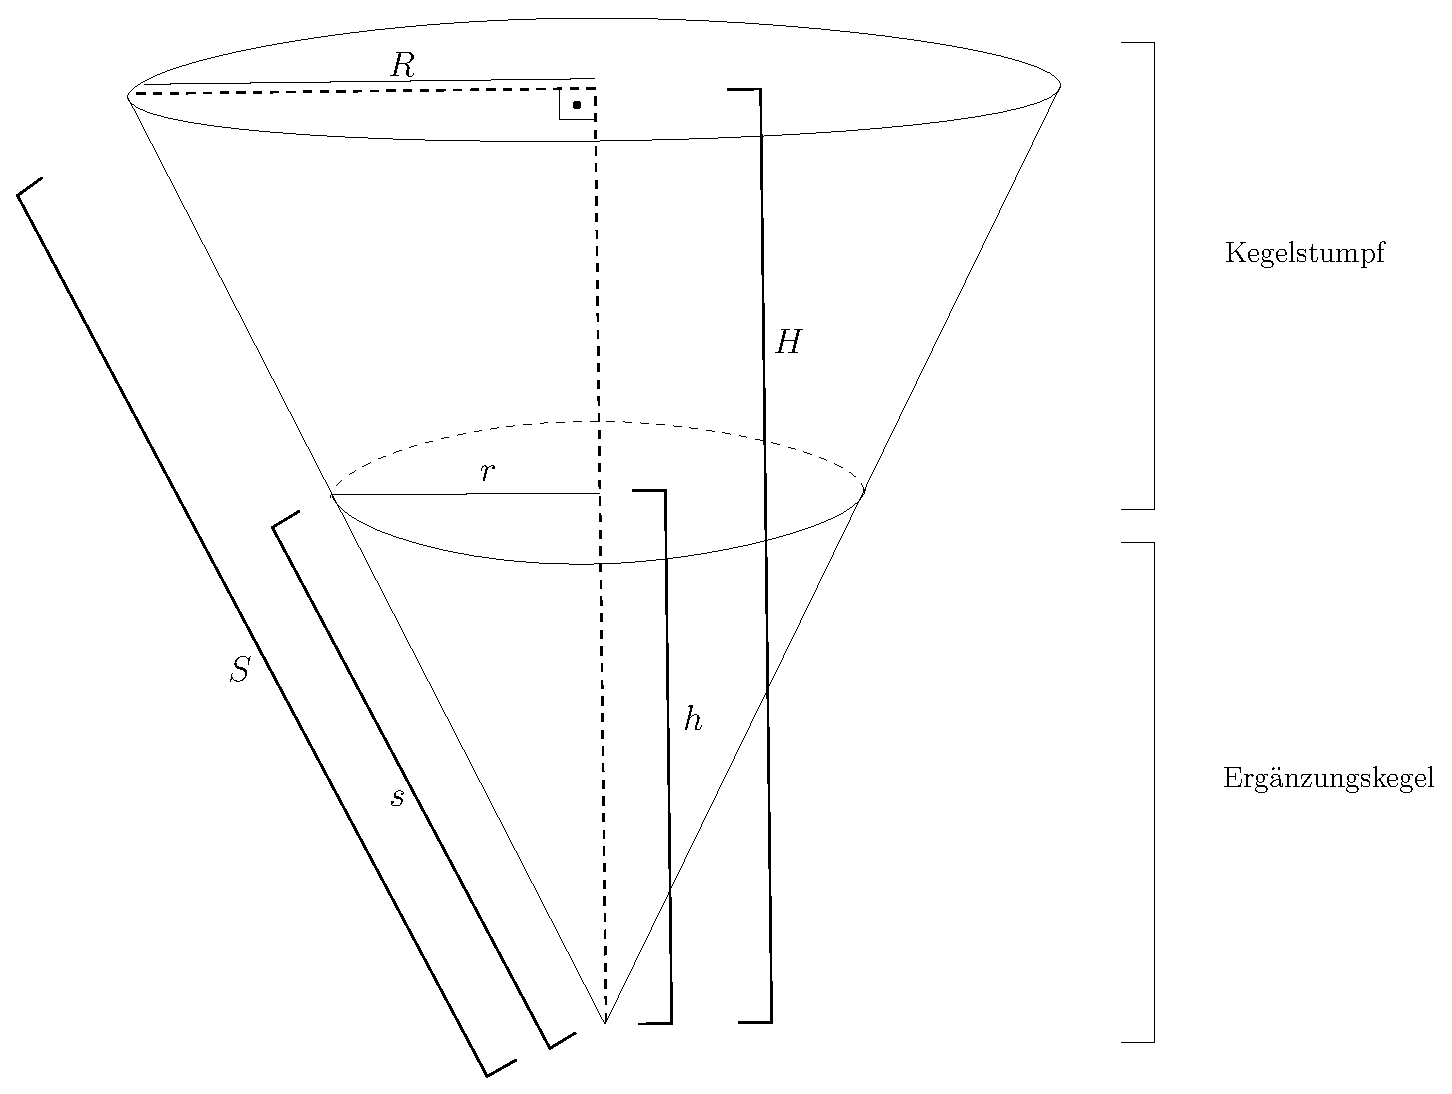
\includegraphics[scale=.5]{images/fullCone3.eps}
	\caption{Kegelstumpfergänzung}
	\label{fig:coneWithFrustum}
\end{figure}
Ein Kegel mit Spitze $K(0,0,0)$, Radius $R$ und Höhe $H$ kann parametrisch beschrieben werden als:
\begin{equation}
\begin{aligned}
x &= \frac{u}{h} R~cos \theta \\
y &= u \\
z &= \frac{u}{h} R~sin \theta
\end{aligned}
\end{equation}
mit $u\in [0, H]$ und $\theta \in [0, 2\pi)$ 

$S$ bezeichnet die Seitenhöhe und ist definiert durch $S = \sqrt{R^2 + H^2}$

\begin{definition}[Kegelstumpf]
	entsteht wenn bla bla 
\end{definition}

\begin{figure}[!htb]
	\centering
	\includegraphics[scale=.7]{images/coneFrustum.eps}
	\caption{Kegelstumpf}
	\label{fig:coneFrustum}
\end{figure}


\begin{equation}
\begin{aligned}
x &= (r + \frac{u}{h} (R - r))~cos \theta \\
y &= u \\
z &= (r + \frac{u}{h} (R - r))~sin \theta
\end{aligned}
\end{equation}
mit $u\in [0, \Delta H]$ und $\theta \in [0, 2\pi)$


\begin{figure}[!htb]
	\centering
	\includegraphics[scale=.4]{images/coneLateral.eps}
	\caption{Kegelmantelfläche}
	\label{fig:coneLateral}
\end{figure}


\begin{equation}
\begin{aligned}
x &= -(s + \lambda (S-s)) ~sin \phi \\
y &= (s + \lambda (S-s)) ~cos \phi
\end{aligned}
\end{equation}
mit $\lambda \in [0, 1]$ und $\phi \in [0, \alpha]$




Sei $\mathcal{R}(y) := r + \frac{y}{h} (R - r)$, $\Phi(x,y,z) := \atant\left(\frac{z}{d(y)}, \frac{x}{d(y)}\right)$, $\mathcal{S}(y) := s + \frac{y}{\Delta H} (S-s)$
\begin{equation}
\begin{aligned}
\Psi \colon [r,R] \times [0, \Delta H] \times [r,R] &\to [s,S] \times [s,S]\\
(x,y,z) &\mapsto \left(-\mathcal{S}(y)\sin \Phi(x,y,z), \mathcal{S}(y)\cos\Phi(x,y,z)\right) 
\end{aligned}
\end{equation}

Sei $\mathcal{R}(y) := r + \frac{y}{h} (R - r)$, $\Phi(x,y,z) := \atant\left(\frac{z}{d(y)}, \frac{x}{d(y)}\right)$, $\mathcal{S}(y) := s + \frac{y}{\Delta H} (S-s)$
\begin{equation}
\begin{aligned}
\Psi^{-1} \colon  [s,S] &\to [r,R] \times [0, \Delta H] \times [r,R]\times [s,S]\\
(x,y,z) &\mapsto \left(-\mathcal{S}(y)\sin \Phi(x,y,z), \mathcal{S}(y)\cos\Phi(x,y,z)\right) 
\end{aligned}
\end{equation}




\section{Ellipse}

\begin{definition}[Ellipse]
	Kegelschnitt und so bla bla
\end{definition}

\begin{figure}[!htb]
	\centering
	\includegraphics[scale=.7]{images/ellipse.eps}
	\caption{Ellipse}
	\label{fig:ellipse}
\end{figure}

\todo{stimmt das mit der ungleichung?}
\begin{equation} 
ax^2 + by^2 + cxy + dx + ey + f = 0 \quad \text{mit}\quad b^2-4ac < 0
\end{equation} 
mit $a,b,c,d,e,f \in \mathbb{R}$ oder

\begin{equation} \label{eq:ellipse1}
\frac{((x - x_0)\cos\theta + (y - y_0)\sin\theta)^2}{a^2} + \frac{((x - x_0)\sin\theta - (y - y_0)\cos\theta)^2}{b^2} = 1
\end{equation} 

\todo{a,b, semi-major?}

beziehungsweise als parametrische Form:

\begin{equation} \label{eq:ellipse2}
\begin{pmatrix}x \\ y\end{pmatrix} = \begin{pmatrix}x_0 + a\cos\phi\cos\theta - b\sin\phi\sin\theta \\ 
y_0 + a\cos\phi\sin\theta + b\sin\phi\cos\theta\end{pmatrix}
\end{equation}
mit $\phi \in [0, 2\pi)$

Diese beiden Formen sind ineinander umformbar. Da wir die Umformung von \ref{eq:ellipse1} nach \ref{eq:ellipse2} später brauchen wird sie hier einmal exemplarisch vorgeführt. 

Zunächst einmal fällt auf, dass der gemischten Term $cxy$ genau dann null ist wenn, die Ellipse nicht rotiert wurde. Im ersten Schritt versuchen wir also die Rotation der Ellipse rückgängig zu machen, um den Rotationswinkel zu bestimmen und anschließend den Ellipsenmittelpunkt ermitteln zu können.

Die Gleichung \ref{eq:ellipse1} kann umgeformt werden zu:
\begin{equation*}
\begin{aligned}
\underbrace{\begin{pmatrix}x & y\end{pmatrix}}_{=:u^T}\begin{pmatrix}a & \frac{c}{2} \\ \frac{c}{2} & b\end{pmatrix}\underbrace{\begin{pmatrix}x \\ y\end{pmatrix}}_{=u} +\begin{pmatrix}d & e\end{pmatrix}\underbrace{\begin{pmatrix}x \\ y\end{pmatrix}}_{=u}+ f = 0 \\
\Leftrightarrow u^TMu +\begin{pmatrix}d & e\end{pmatrix}u + f = 0 \\
\end{aligned}
\end{equation*} 
Der gemischte Term wird alleine durch $M = \begin{pmatrix}a & \frac{c}{2} \\ \frac{c}{2} & b\end{pmatrix}$ bestimmt. Da die Matrix $M$ symmetrisch ist, ist sie orthogonal diagonalisierbar. Insbesondere sind die Eigenvektoren zueinander orthogonal.

Es gilt $M = S^TDS$, wobei $S\in\mathbb{R}^{2\times2}$ eine orthogonale Matrix mit den normierten Eigenvektoren als Zeilen und $D = \text{diag}(\lambda_1, \lambda_2)\in\mathbb{R}^{2\times2}$ eine Diagonalmatrix mit den beiden Eigenwerten von $M$ auf der Diagonalen ist. Ohne Beschränkung der Allgemeinheit gelte $\lambda_1 <= \lambda_2$, andernfalls vertausche die Eigenvektoren in $S$. 

Sei nun $v := Su$
Insgesamt gilt also:

\begin{equation*} \label{eq:PCARot}
\begin{aligned}
&u^T(S^TDS)u +\begin{pmatrix}d & e\end{pmatrix}\underbrace{(S^TS)}_{=\ind}u + f = 0 \\
\Leftrightarrow\quad &(u^TS^T)D(Su) +\begin{pmatrix}d & e\end{pmatrix}S^T(Su) + f = 0 \\
\Leftrightarrow\quad &v^{T}Dv +\begin{pmatrix}d & e\end{pmatrix}S^Tv + f = 0 
\end{aligned}
\end{equation*}

Man kann leicht nachrechnen, dass der gemischte Teil somit eliminiert wurde. Durch Anwenden der Transformation $S$ wurde $u$ also in das Koordinatensystem der Ellipse transformiert.

Eine Rotationsmatrix mit Rotationswinkel $\theta$ in 2D ist definiert durch: 
\begin{equation}
\begin{aligned}
R = \begin{pmatrix}\cos\theta & -\sin\theta \\ \sin\theta & \cos\theta\end{pmatrix}
\end{aligned}
\end{equation}

Es gilt offenbar $S = R$ für ein geeignetes $\theta$, da die Eigenvektoren zueinander orthogonal sind. $\theta$ kann also einfach ausgerechnet werden, denn es gilt:

\begin{equation*}
\theta = \atant(\sin\theta, \cos\theta) = \atant(S_{2,1}, S_{1,1})
\end{equation*}

Multipliziert man nun \ref{eq:PCARot} aus ergibt sich:

\begin{equation*}
\begin{aligned}
&\lambda_1v_1^2 + \lambda_2v_2^2 + \underbrace{\begin{pmatrix}d & e\end{pmatrix}S^T}_{=:(d', e')}v + f = 0 \\
\Leftrightarrow\quad &\lambda_1v_1^2 + \lambda_2v_2^2 + d'v_1 + e'v_2 + f = 0 \\
\Leftrightarrow\quad &(\lambda_1v_1^2 + d'v_1)+ (\lambda_2v_2^2 + e'v_2) + f = 0 \\
\Leftrightarrow\quad &(\lambda_1v_1^2 + d'v_1) + (\frac{d'^2}{4\lambda_1} - \frac{d'^2}{4\lambda_1}) + (\lambda_2v_2^2 + e'v_2) + (\frac{e'^2}{4\lambda_2} - \frac{e'^2}{4\lambda_2}) + f = 0 \\
\Leftrightarrow\quad &\left[\lambda_1\left(v_1^2 + \frac{2d'}{2\lambda_1}v_1 + \frac{d'^2}{4\lambda_1^2}\right) - \frac{d'^2}{4\lambda_1}\right] +\left[\lambda_2\left(v_2^2 + \frac{2e'}{2\lambda_2}v_2 + \frac{e'^2}{4\lambda_2^2}\right) - \frac{e'^2}{4\lambda_2}\right] + f = 0 \\
\Leftrightarrow\quad &\lambda_1(v_1 + \underbrace{\frac{d'}{2\lambda_1}v_1}_{ = -x'_0})^2 +\lambda_2(v_2 + \underbrace{\frac{e'}{2\lambda_2}v_2}_{ = -y'_0})^2 - \underbrace{(\frac{d'^2}{4\lambda_1} + \frac{e'^2}{4\lambda_2} - f)}_{=:\sigma} = 0
\end{aligned}
\end{equation*}

, da $\lambda_1, \lambda_2 > 0$, da symmetrisch und so. Das Zentrum der transformierten Ellipse kann einfach abgelesen werden. Um das Zentrum der eigentlichen Ellipse zu bestimmen, muss mit der inversen Rotation also $S^T$ multipliziert werden. Obige Gleichung lässt sich weiter vereinfachen: 


\begin{equation} \label{eq:PCAKoeff}
\begin{aligned}
&\lambda_1(v_1 -x'_0)^2 +\lambda_2(v_2 -y'_0)^2 = \sigma \\
\Leftrightarrow\quad & \frac{\lambda_1}{\sigma}(v_1 -x'_0)^2 +\frac{\lambda_2}{\sigma}(v_2 -y'_0)^2  =1
\end{aligned}
\end{equation}

Vergleicht man nun \ref{eq:PCAKoeff} mit \todo{noch ohne rotation einfügen} so sieht man das:
bla bla 
gelten muss






\newpage
ellipse distanz mit transformationen die nötig sind

Hauptachsentransformation

schnittpunkt linie ellipse


\section{Parameterschätzung}

Hough?
Paremterschätzung Ransac. anzahl interationen




\section{Kamerakalibrierung}

kamerakalibrierung

projektionsmatrix
(homogene Koordinaten????)
SVD, QR, LSQ?



Kantendetektion (canny sobel)

\section{Deformable Templates}


deformable templates

evtl noch am ende delaunay